\documentclass[crop,tikz]{standalone}
\usetikzlibrary{mindmap}
%\setlength\parindent{0pt}
\renewcommand{\footnotesize}{\fontsize{5.5}{6.0}\selectfont}
\renewcommand{\normalsize}{\fontsize{7.5}{11.0}\selectfont}
\begin{document}
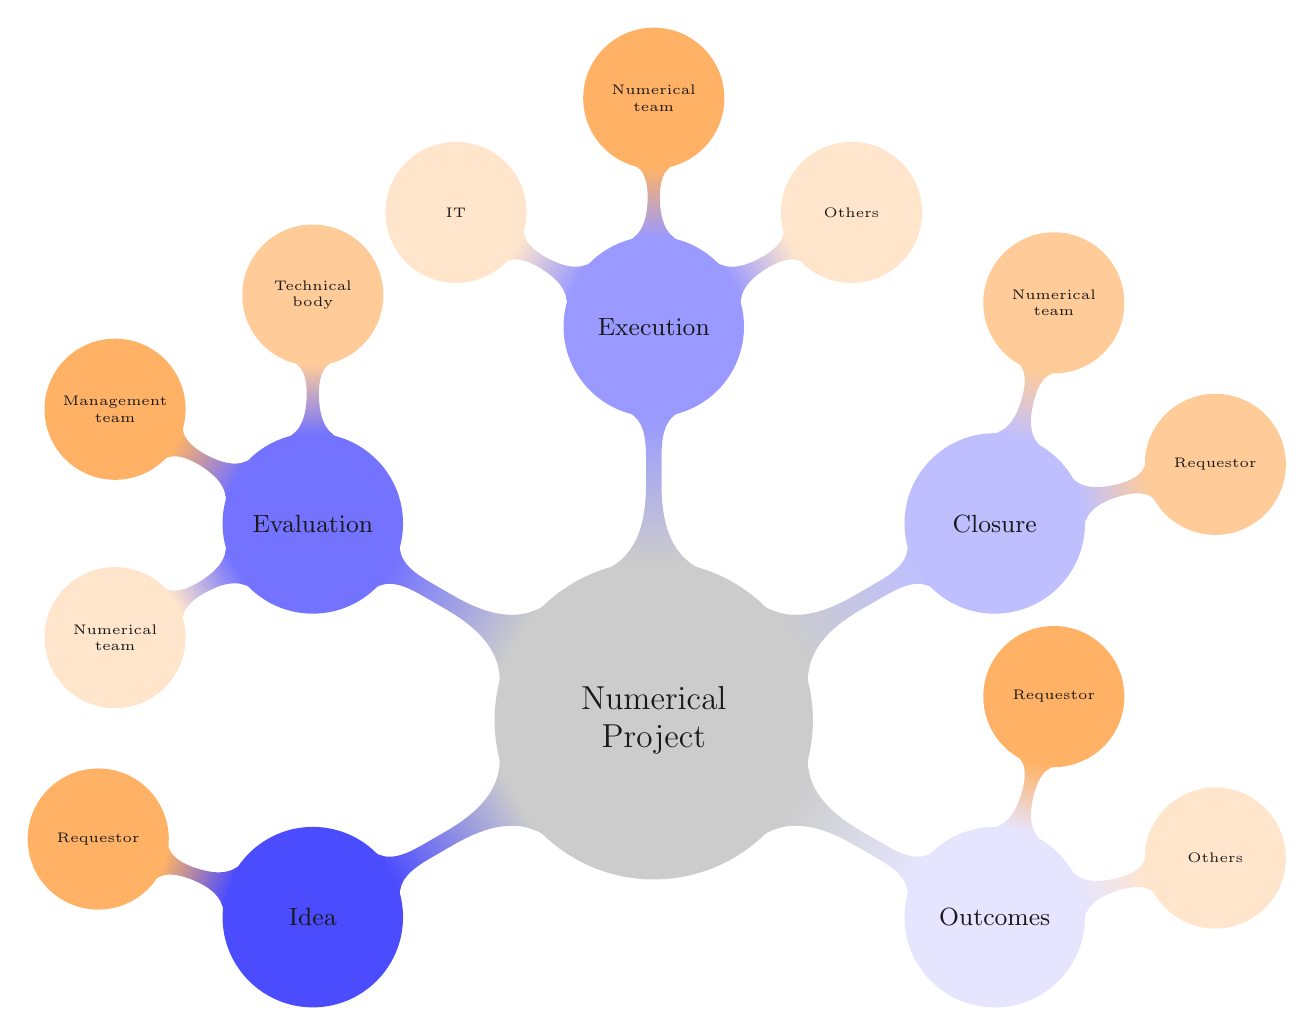
\begin{tikzpicture}
	\path[
		mindmap,
		concept color=gray!40,
		text=black!90
	] {
		node[concept] {Numerical\\Project} [clockwise from=210]
		child[concept color=blue!70]  { 
			node[concept] {Idea} [clockwise from=160]
			child[concept color=orange!60] { node[concept] {Requestor}  }
		}
		child[concept color=blue!55]  { 
			node[concept] {Evaluation} [clockwise from=210]
			child[concept color=orange!20] { node[concept] {Numerical team} }
			child[concept color=orange!60] { node[concept] {Management team}  }
			child[concept color=orange!40] { node[concept] {Technical body}  }
		}
		child[concept color=blue!40]   {
			node[concept] {Execution} [clockwise from=150]
			child[concept color=orange!20] { node[concept] {IT}  }
			child[concept color=orange!60] { node[concept] {Numerical team} }
			child[concept color=orange!20] { node[concept] {Others}  }
		}
		child[concept color=blue!25]   {
			node[concept] {Closure} [clockwise from=75]
			child[concept color=orange!40] { node[concept] {Numerical team} }
			child[concept color=orange!40] { node[concept] {Requestor}  }
		}
		child[concept color=blue!10]   {
			node[concept] {Outcomes} [clockwise from=75]
			child[concept color=orange!60] { node[concept] {Requestor}  }
			child[concept color=orange!20] { node[concept] {Others} }
		}
	};
\end{tikzpicture}
\end{document}